\section{Ferramenta Construída}

A ferramenta desenvolvida (no qual está disponível no seguinte endereço https://github.com/iamPedroVictor/LSystem2Unity) possui um editor customizado que o torna mais amigável para o desenvolvedor, podendo construir suas estruturas com o L-Sistema, ela conta com:
\begin{itemize}
	\item LSystem - Componente principal, aonde faz o processamento das estruturas com as regras de produção.
	\item TurtleAgent - Componente para leitura da estrutura fornecida pelo LSystem.
	\item Ruleset - Estrutura que armazena as regras de produção que vão ser utilizadas pelo LSystem.
\end{itemize}

\subsection{Fluxo da ferramenta}
Em seu atual momento a ferramenta começa seu processo assim que a função Start do MonoBehaviour é chamado, seu fluxo pode ser visto pelo diagrama na figura \ref{LSystemFlow}

\begin{figure}[!h]
	\centering
	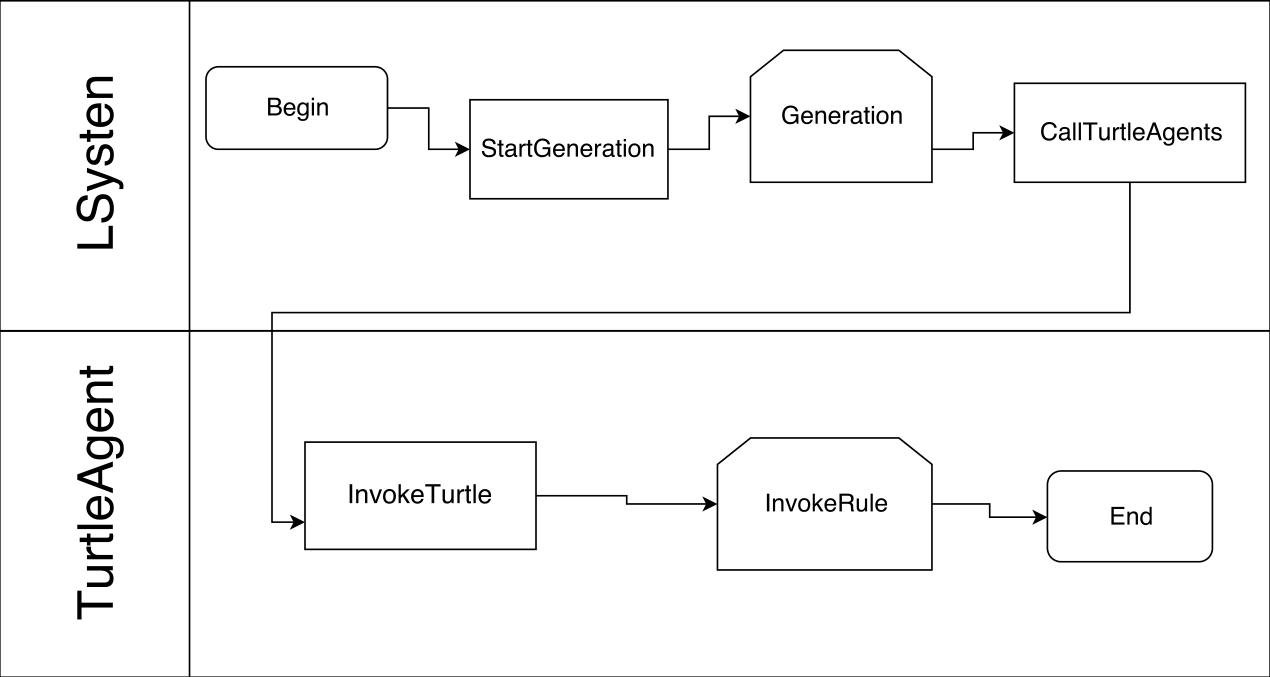
\includegraphics[width=0.4\textwidth]{LSystemFlow}
	\caption{Fluxo da ferramenta LSystem2Unity}
	\label{LSystemFlow}
\end{figure}

\subsection{Interface da ferramenta}
O componente principal para a geração das estruturas esta no monobehaviour LSystem demostrado na figura \ref{LSystemComponent}, nele tem as propriedades principais, além do campo para por uma lista de regras de substituição.

\begin{figure}[!h]
	\centering
	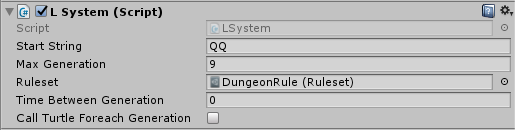
\includegraphics[width=0.4\textwidth]{LSystemComponent}
	\caption{Interface do componente LSystem}
	\label{LSystemComponent}
\end{figure}

A figura \ref{LRuleSet} apresenta a interface de Ruleset já customizada, aonde o usuário pode ver com mais facilidade os símbolos que vão ser trocados, além de botões para adicionar e remover novas regras.
\begin{figure}[!h]
	\centering
	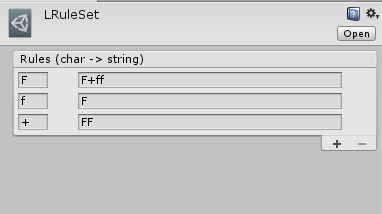
\includegraphics[width=0.4\textwidth]{LRuleEditor}
	\caption{Interface de Ruleset}
	\label{LRuleSet}
\end{figure}

 A interface do componente TurtleAgent possui a mesma semelhança, mas para facilitar a leitura do componente, há uma funcionalidade de mostrar o conteúdo presente na lista somente quando o item for selecionado, isso é demostrado nas figuras \ref{TurtleAgentWithout} e \ref{TurtleAgentSelect}, com o item não selecionado e selecionado respectivamente.

\begin{figure}[!h]
	\centering
	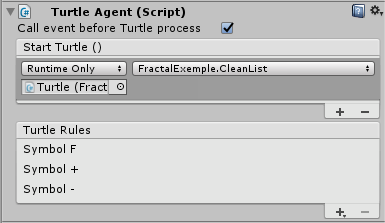
\includegraphics[width=0.3\textwidth]{TurtleAgentInspectorNoSelected}
	\caption{Interface de TurtleAgent sem item selecionado}
	\label{TurtleAgentWithout}
\end{figure}

\begin{figure}[!h]
	\centering
	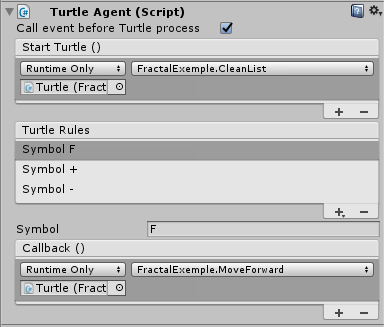
\includegraphics[width=0.3\textwidth]{TurtleAgentInspectorSelected}
	\caption{Interface de TurtleAgent com item selecionado}
	\label{TurtleAgentSelect}
\end{figure}